\documentclass[conference]{IEEEtran}
\usepackage{amsmath,amssymb,bm,booktabs}
\usepackage{graphicx,balance}
\usepackage{tikz}
\usetikzlibrary{arrows.meta,calc,positioning,shapes.geometric}
% Generated by scripts/build_spring_story.py; no manually chosen result values.
\newcommand{\DivSaving}{1.319}
\newcommand{\DivPayloadSaving}{0.758}
\newcommand{\DivTotalSaving}{0.353}
\newcommand{\DivRequestSaving}{1.784}
\newcommand{\DivAdaptiveNack}{73.970}
\newcommand{\DivFlowNack}{72.651}
\newcommand{\KodSaving}{1.453}
\newcommand{\KodPayloadSaving}{0.846}
\newcommand{\KodTotalSaving}{0.391}
\newcommand{\KodRequestSaving}{2.026}
\newcommand{\KodAdaptiveNack}{71.701}
\newcommand{\KodFlowNack}{70.249}

\title{Compute Before Retransmit: Reliability-Anchored\\Flow Matching for DeepJSCC HARQ}
\author{\IEEEauthorblockN{Anonymous Authors}\IEEEauthorblockA{Author information withheld in this draft}}
\begin{document}
\maketitle
\begin{abstract}
Can a receiver improve its current estimate enough to avoid another physical
transmission? We study this question for image DeepJSCC with two-round,
quality-based hybrid automatic repeat request (HARQ). FlowHARQ repairs selected
latent tokens through conditional flow matching, preserves unselected tokens,
and applies a separately calibrated quality decision. A fixed codec and common
maximum-ratio-combining fallback isolate the effect of receiver computation.
On DIV2K and Kodak24, an existing ten-run extension reduces NACK probability
by 1.319 and 1.453 percentage points, respectively, within predefined mean
PSNR and LPIPS tolerances. A paired decision decomposition shows that quality
improvement on already-accepted images offsets degradation on saved rounds;
the aggregate is not a per-image improvement. Charging token-scale metadata
and reliable feedback reduces payload savings of 0.758\% and 0.846\% to
0.353\% and 0.391\%. Substantial false acceptance and final outage remain.
A paired published-SwinJSCC transfer test also exposes a large codec-quality
gap. The evidence supports a small within-codec tradeoff, not reliable
target-quality delivery or a competitive end-to-end HARQ system.
\end{abstract}
\begin{IEEEkeywords}
DeepJSCC, HARQ, flow matching, semantic communication, receiver processing.
\end{IEEEkeywords}

\section{Introduction}
Deep joint source--channel coding (DeepJSCC) produces a reconstruction even
when channel conditions do not support high image quality \cite{deepjscc}.
A receiver must therefore decide whether to accept that reconstruction or
request additional symbols. This decision has two distinct failure modes:
requesting a transmission that local processing could avoid, and accepting an
image whose quality falls below the service target. Reducing the first without
measuring the second can make an overconfident receiver appear efficient.

We investigate a receiver action between equalization and ACK/NACK: refine
the received latent representation, then reassess whether a physical round is
needed. The action adds computation but no channel observation. It is useful
only if its change in the final decision compensates for its processing cost
without an unacceptable quality loss. Image restoration quality alone cannot
establish this communication benefit.

\textit{Position relative to prior work.}
DeepJSCC-f uses channel-output feedback to encode further information
\cite{deepjscc_f}, while SAFG-HARQ changes retransmission granularity
\cite{fineharq}. These approaches modify physical information delivery.
CDDM instead uses diffusion for channel denoising \cite{cddm}; FlowSem and
realization-coupled flow matching study generative refinement in communication
\cite{flowsem,rcbfm}, and generative semantic HARQ has been investigated for
text latents \cite{genharq}. In computer vision, FlowIE studies conditional
rectified flow for efficient enhancement \cite{Zhu_2024_CVPR}; ResFlow models
restoration through an augmented degradation flow \cite{Qin_2025_CVPR}.
These works motivate iterative refinement, but their restoration results do
not establish safe early acceptance on a wireless link. Our question concerns
the subsequent communication decision, not priority for applying flow matching.

FlowHARQ constrains repair with a reliability mask, then decides on the repaired
state. On NACK, it uses the same two-observation MRC fallback as the no-repair
policy. When both retransmit, their delivered images are identical.

The paper makes three contributions. First, it specifies this receiver action
with explicit forward symbols, side information, and binary feedback. Second,
it separates changes in accepted-image quality from changes due to saved or
additional rounds through a paired decision decomposition. Third, it evaluates
the resulting tradeoff using frozen experiments, a finite-precision audit,
and charged signaling costs. The benefit is modest and does not establish
reliable 24-dB delivery. We report that boundary alongside the saving rather
than equating an average-quality tolerance with a reliability guarantee.

\begin{figure}[t]
\centering
\resizebox{.93\columnwidth}{!}{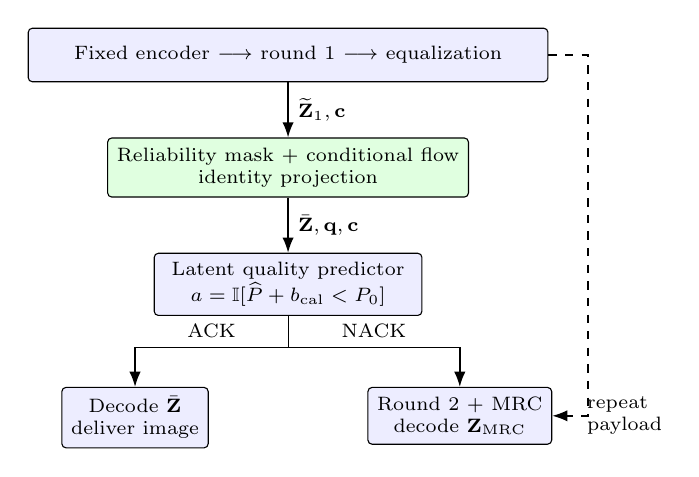
\begin{tikzpicture}[
  font=\scriptsize,
  node distance=7mm and 5mm,
  block/.style={draw, rounded corners=1.5pt, minimum height=6.8mm,
                minimum width=16mm, align=center, fill=blue!7},
  decision/.style={draw, diamond, aspect=2.1, align=center, fill=orange!12,
                   inner sep=1.1pt},
  arrow/.style={-Latex, line width=.55pt},
  repair/.style={draw, rounded corners=1.5pt, minimum height=7.5mm,
                 minimum width=20mm, align=center, fill=green!12},
]
\node[block, minimum width=66mm] (ch1)
 {Fixed encoder $\longrightarrow$ round 1 $\longrightarrow$ equalization};
\node[repair, below=of ch1, minimum width=34mm] (fm)
 {Reliability mask + conditional flow\\identity projection};
\node[block, below=of fm, minimum width=34mm] (quality)
 {Latent quality predictor\\$a=\mathbb I[\widehat P+b_{\rm cal}<P_0]$};
\node[block, below left=9mm and -7mm of quality] (accept)
 {Decode $\bar{\mathbf Z}$\\deliver image};
\node[block, below right=9mm and -7mm of quality] (ch2)
 {Round 2 + MRC\\decode $\mathbf Z_{\rm MRC}$};
\draw[arrow] (ch1) -- node[right]{$\widetilde{\mathbf Z}_1,\mathbf c$} (fm);
\draw[arrow] (fm) -- node[right]{$\bar{\mathbf Z},\mathbf q,\mathbf c$} (quality);
\coordinate (split) at ($(quality.south)+(0,-4mm)$);
\draw (quality.south) -- (split);
\draw[arrow] (split) -| node[pos=.25,above]{ACK} (accept.north);
\draw[arrow] (split) -| node[pos=.25,above]{NACK} (ch2.north);
\draw[arrow, dashed] (ch1.east) -- ++(5mm,0) |-
 node[pos=.65,right,align=left]{repeat\\payload} (ch2.east);
\end{tikzpicture}
}
\caption{Receiver computation precedes the physical retransmission decision.
Both policies use the same first observation and identical MRC fallback. The
dashed path carries the original payload, not newly generated information.}
\label{fig:system}
\end{figure}

\section{System Model and Evaluation Objective}
\subsection{Two-Round Image Link}
For an RGB image $\mathbf x\in[0,1]^{H\times W\times3}$, a fixed encoder
produces $\mathbf Z=E_\theta(\mathbf x)\in\mathbb R^{N\times d}$.
Pairing real features forms $d/2$ complex symbols $\mathbf z_i^c$ per token.
The transmitted token is $\mathbf s_i=\mathbf z_i^c/\alpha_i$, where
$\alpha_i=(2\|\mathbf z_i^c\|^2/d+\epsilon)^{1/2}$ and $\epsilon=10^{-8}$.
For $N=256$, $d=32$, and $H=W=256$, each round carries $B=Nd/2=4096$
complex payload symbols, giving a payload channel-bandwidth ratio of $1/48$.

Round $r\in\{1,2\}$ yields $\mathbf y_r=h_r\mathbf s+\mathbf n_r$, with
$\mathbf n_r\sim\mathcal{CN}(0,10^{-\gamma/10}\mathbf I)$ at nominal SNR
$\gamma$ dB. One flat-fading coefficient applies to the image. Equalization
uses perfect instantaneous CSI and restores the token scales:
\begin{equation}
 \widetilde{\mathbf z}_{r,i}^{c}
 =\alpha_i\frac{h_r^*\mathbf y_{r,i}}{|h_r|^2+\epsilon}.
 \label{eq:equalize}
\end{equation}
The original experiment uses exact scales. Our signaling audit charges
$Q_{16}(\alpha_i)$, an IEEE binary16 value, transmitted once and reused if the
same payload is retransmitted; the finite-precision check replaces $\alpha_i$
by $Q_{16}(\alpha_i)$ in the receiver restoration only.

The two rounds follow a correlated Rayleigh law,
\begin{equation}
 h_2=\rho_\Delta h_1+\sqrt{1-\rho_\Delta^2}\,e,\quad
 \rho_\Delta=J_0(2\pi v f_c\Delta/c),
 \label{eq:channel}
\end{equation}
where $h_1,e\sim\mathcal{CN}(0,1)$ independently, $v$ is speed in m/s,
$f_c=5.9$ GHz, and $\Delta=1$ ms. Speed changes inter-round correlation,
not the marginal first-round fading law. Context $\mathbf c$ comprises SNR,
speed, CSI age and its Jakes correlation, instantaneous gain, and effective
SNR. CSI age is a conditioning variable, not simulated estimation error.

A NACK requests the same normalized payload and produces
\begin{equation}
 \mathbf Z_M=
 \frac{|h_1|^2\widetilde{\mathbf Z}_1+|h_2|^2\widetilde{\mathbf Z}_2}
 {|h_1|^2+|h_2|^2},
 \label{eq:mrc}
\end{equation}
with numerical denominator protection in code. The decoder $D_\theta$ delivers
an accepted first-round state or $D_\theta(\mathbf Z_M)$. No third round is
allowed. ACK/NACK is reliable; this is image-quality HARQ, not CRC-based
error detection. The target $P_0=24$ dB need not be attained after the last
allowed round.

\subsection{Charged Channel Uses and Quality Constraints}
Let $a=1$ denote a NACK. With metadata and feedback efficiencies
$\eta_s,\eta_f$ measured in information bits per complex channel use, define
\begin{equation}
 C(a)=B(1+a)+\left\lceil\frac{16N}{\eta_s}\right\rceil
       +(1+a)\left\lceil\frac{1}{\eta_f}\right\rceil.
 \label{eq:cost}
\end{equation}
The last term charges the initial ACK/NACK and a final ACK when a second
round occurs. Metadata is reused rather than retransmitted. These are charged
uses under ideal reliable signaling, not a complete air-interface budget:
pilots, framing, feedback delay, and control decoding errors are excluded.

Relative to a fixed adaptive-HARQ policy $A$, we evaluate receiver policy $F$
by the design objective
\begin{align}
 \min_F\;&\mathbb E[C(a_F)]\nonumber\\
 \text{s.t. }&\mathbb E[P_A-P_F]\leq0.02~\mathrm{dB},\quad
              \mathbb E[L_F-L_A]\leq0.003,
 \label{eq:objective}
\end{align}
where $P$ and $L$ are delivered-image PSNR and LPIPS \cite{lpips}. This is an
evaluation criterion, not a claim that our staged training solves a constrained
optimum. Neither average tolerance supplies an image-wise outage guarantee.
Writing $p_j=\Pr(a_j=1)$ and $b_f=\lceil1/\eta_f\rceil$, the exact accounting
identity is
\begin{equation}
 \mathbb E[C(a_A)-C(a_F)]=(B+b_f)(p_A-p_F).
 \label{eq:identitycost}
\end{equation}
Fixed metadata cancels in the absolute difference but dilutes relative savings
through the denominator. Thus $p_A-p_F$, $(p_A-p_F)/p_A$, and
$(p_A-p_F)/(1+p_A)$ represent different quantities: an absolute NACK change,
a relative reduction in requests, and a relative payload saving.

\subsection{What a Saved Round Does and Does Not Establish}
Let $P_D,P_R,P_M$ denote the PSNR of direct, repaired, and MRC images for
the same source and physical observations. With $I_{uv}=\mathbb I[a_A=u,a_F=v]$,
the delivered-quality difference obeys the sample-wise identity
\begin{align}
 P_F-P_A={}&I_{00}(P_R-P_D)+I_{10}(P_R-P_M)\nonumber\\
          &+I_{01}(P_M-P_D).
 \label{eq:decomposition}
\end{align}
This follows by enumerating the four decision pairs; the $I_{11}$ term is
zero because the fallback is common. The same identity holds for any scalar
reconstruction metric, including MSE and LPIPS, with their respective signs.
An overall PSNR gain can therefore coexist with a loss on the saved-round
subset. We evaluate both the net change and its components.

For reliability, define ACK coverage $\kappa_j=\Pr(a_j=0)$, joint false ACK
$u_j=\Pr(a_j=0,P_j<P_0)$, and conditional false ACK
$r_j=u_j/\kappa_j$ when $\kappa_j>0$. Final outage is
$o_j=\Pr(P_j<P_0)$, including delivery after MRC. Neither
\eqref{eq:objective} nor the cost identity bounds $r_j$ or $o_j$.
When $\kappa_j=0$, conditional false ACK is undefined, not evidence of a
useful zero-risk service. These quantities distinguish economical decisions
from reliable delivery.

\section{Reliability-Anchored FlowHARQ}
\subsection{Repair Only the Selected Latent Coordinates}
A reliability head predicts $q_i=g_q(\widetilde{\mathbf z}_{1,i},\mathbf c)$,
and inference selects $m_i=\mathbb I[q_i\geq\tau_r]$. During training only,
an oracle mask $m_i^*$ selects the largest $\lceil0.35N\rceil$ clean-to-received
token errors and supervises a balanced binary cross-entropy loss. Neither the
clean image nor this oracle mask is available to the deployed receiver.

Following conditional flow matching \cite{flowmatching}, let
$\mathbf u_i=\mathbf z_i-\widetilde{\mathbf z}_{1,i}$ and sample
$t\sim\mathcal U[0,1]$ on the path
$\mathbf z_i(t)=\widetilde{\mathbf z}_{1,i}+tm_i^*\mathbf u_i$.
The velocity network sees this state, time, receiver context, the received
tokens, and a pooled anchor from unselected tokens. To avoid domination by
large zero-forcing residuals in deep fades, its regression loss is
\begin{align}
 \mathcal L_{\rm FM}=\mathbb E_t
 \frac{\sum_i m_i^*d^{-1}\sum_j
 \rho_{0.1}((v_{\psi,ij}-u_{ij})/s_i)}{\max(1,\sum_i m_i^*)},\nonumber\\
 s_i=\max(1,\|\mathbf u_i\|/\sqrt d),
 \label{eq:fm}
\end{align}
where $\rho_{0.1}$ is smooth-$L_1$ and $s_i$ is detached. An image $L_1$
loss on decoded repair aligns transport with the fixed decoder. That branch
uses the predicted hard mask with a straight-through gradient; it does not
use the oracle mask from velocity supervision.

At inference, $K=4$ explicit updates start from
$\mathbf Z^{(0)}=\widetilde{\mathbf Z}_1$:
\begin{equation}
 \mathbf Z^{(k+1)}=\mathbf Z^{(k)}+
 \frac{\mathbf m}{K}\odot
 v_\psi(\mathbf Z^{(k)},(k+\tfrac12)/K;
       \widetilde{\mathbf Z}_1,\mathbf m,\mathbf c).
 \label{eq:flow}
\end{equation}
Mid-interval time inputs do not make this a second-order midpoint solver.
The output projection
$\bar{\mathbf z}_i=(1-m_i)\widetilde{\mathbf z}_{1,i}+m_i\mathbf z_i^{(K)}$
preserves every unselected latent token exactly. It does not preserve spatial
image regions, since decoding mixes tokens. Likewise, the dense Transformer
still processes all tokens; masking constrains content changes rather than
delivering sparse-computation savings.

\subsection{Decide on the Repaired State, Fall Back to Physical Evidence}
A quality head estimates log-MSE from the latent, reliability scores, and
context. Its converted PSNR prediction $\widehat P$ is trained on direct and
repaired states using log-MSE regression and a boundary loss
\begin{equation}
 \mathcal L_q^{\rm boundary}=\operatorname{BCEWithLogits}
 \big((P_0-\widehat P)/T_q,\mathbb I[P<P_0]\big).
 \label{eq:quality}
\end{equation}
The true quality on the right is training supervision only. A separate
decision-training stage freezes the codec, reliability head, and velocity
field. Scalar biases $b_A,b_F$ are subsequently fitted on calibration images,
giving $a_A=\mathbb I[\widehat P(\widetilde{\mathbf Z}_1)+b_A<P_0]$ and
$a_F=\mathbb I[\widehat P(\bar{\mathbf Z})+b_F<P_0]$.
On ACK, FlowHARQ decodes $\bar{\mathbf Z}$; on NACK it decodes
\eqref{eq:mrc}. The baseline uses the direct state on ACK. Separate calibration
is necessary because repair changes the predictor's input distribution;
calibration does not, by itself, certify a false-ACK bound.

\begin{figure*}[t]
\centering
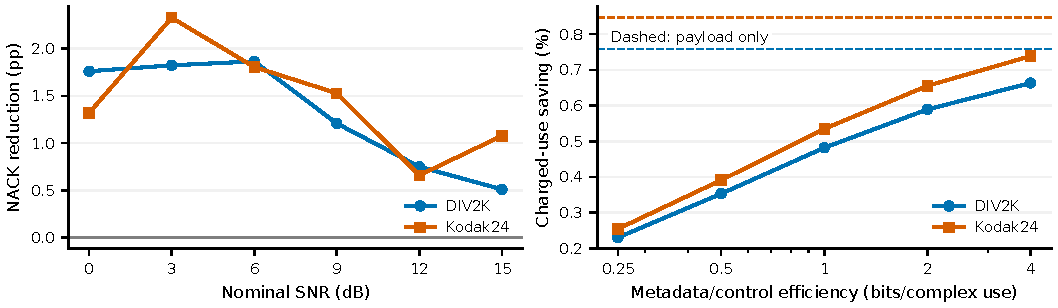
\includegraphics[width=\textwidth]{figures/spring_audit.pdf}
\caption{Frozen ten-run extension, uniformly averaged over images, four speeds,
and three channel draws per trained receiver. Left: paired NACK reduction by
SNR. Right: relative saving after charging binary16 token scales once and
reliable control at $\eta_s=\eta_f$; dashed lines show payload-only savings.
The right panel re-accounts archived decisions and is not a new quantized-model
performance experiment. All efficiency points are reported.}
\label{fig:audit}
\end{figure*}

\section{Experimental Results}
\subsection{Protocol and Comparisons}
We test request savings, their decision-level mechanism, and their reliability
and signaling costs.
The fixed Swin-based codec has 21.83M parameters, while the reliability,
velocity, and quality heads add 0.479M. The velocity field has two Transformer
blocks, width 128, and four attention heads. Receiver training uses DIV2K
\cite{div2k} random $256\times256$ crops for 40 epochs, followed by ten
quality-head epochs. AdamW uses batch size 2, learning rate $2\times10^{-4}$
for repair and $10^{-4}$ for the quality-only stage, weight decay $10^{-4}$,
and gradient clipping at 5. The boundary temperature is 1 dB, with equal
regression and classification weights. Training samples SNR
uniformly over 0--15 dB, speed over 0--120 km/h, and CSI age over 0--5 ms.
Calibration fixes $K=4$, $\tau_r=0.8$, $P_0=24$ dB, and the quality biases
using the first 20 DIV2K validation images. The remaining 80 images are held
out; Kodak24 receives no recalibration. Test images are center-cropped to
$256\times256$ RGB. Tests span SNRs $\{0,3,6,9,12,15\}$ dB and speeds
$\{30,60,90,120\}$ km/h, with CSI age fixed at 2 ms.

The original confirmation comprises three trained receivers and three channel
seeds per receiver. A previously locked extension increases the receiver count
to ten; it is reported separately, not relabeled as the original experiment.
No additional training or seed sweep is performed for this paper revision.
Each policy is evaluated on paired images and physical channel observations.
Confidence intervals in Table~\ref{tab:main} use paired per-training-run
differences with a Student-$t$ interval, averaging channel draws within each
run. Repeated channel draws are not counted as independent training runs.

Controlled comparisons comprise direct one-round decoding, always-two-round
MRC, repair without HARQ, adaptive HARQ without repair, and FlowHARQ. These
isolate the receiver decision with identical codec and channel resources.
They are not independent published architectures. Published author-model
references are treated separately below because feedback, training, and
channel assumptions differ.

\begin{table}[t]
\caption{Paired FlowHARQ minus adaptive HARQ. Positive saving means fewer NACKs;
positive $\Delta$LPIPS means worse perceptual distance. Original and extended
cohorts are separated. PSNR is in dB.}
\label{tab:main}
\centering
\resizebox{\columnwidth}{!}{\begin{tabular}{llrrr}
\toprule
Dataset & Runs & Saving (pp) [95\% CI] & $\Delta$PSNR & $\Delta$LPIPS \\
\midrule
DIV2K & 3 & 1.296 [0.023, 2.570] & +0.0206 & +0.00132 \\
DIV2K & 10 & 1.319 [1.102, 1.537] & +0.0144 & +0.00143 \\
Kodak24 & 3 & 2.025 [0.708, 3.343] & +0.0284 & +0.00128 \\
Kodak24 & 10 & 1.453 [1.081, 1.825] & +0.0253 & +0.00131 \\
\bottomrule
\end{tabular}
}
\end{table}

\subsection{Does Receiver Repair Reduce Physical Requests?}
Table~\ref{tab:main} separates the original result from the ten-run extension.
In the latter,
DIV2K NACK probability changes from \DivAdaptiveNack\% to \DivFlowNack\%,
and Kodak24 from \KodAdaptiveNack\% to \KodFlowNack\%. Mean delivered PSNR
changes by $+0.0144$ and $+0.0253$ dB, respectively. LPIPS changes by
$+0.00143$ and $+0.00131$: both are within the 0.003 tolerance, but neither
is a perceptual improvement. Fig.~\ref{fig:audit} gives the SNR dependence
rather than presenting the aggregate as a uniform gain.

\subsection{Where Does the Gain Come From?}
To locate the effect, partition paired samples by $(a_A,a_F)$. The identity
$p_A-p_F=\Pr(1,0)-\Pr(0,1)$ separates saved from newly requested rounds.
On DIV2K, 1.4740\% of samples save a round and 0.1545\% request an extra one,
leaving the net 1.3194-point reduction. Both receivers accept 25.8750\% and
both request retransmission on 72.4965\%. In the last group the delivered
images are identical, because both use the same MRC observation.

Equation~\eqref{eq:decomposition} explains the quality result. DIV2K samples accepted by
both policies contribute $+0.02719$ dB to the overall mean PSNR difference;
saved-round samples contribute $-0.01332$ dB, and extra-round samples
$+0.00054$ dB. Thus the net PSNR gain does not mean that skipping a physical
observation improves its reconstruction. It combines a quality benefit on
already-accepted images with a small quality sacrifice on saved rounds.
Kodak24 has the same structure: 1.5856\% saved rounds versus 0.1331\% extra
rounds. This is an average resource--quality tradeoff, not per-image dominance.

\subsection{Does the Saving Imply Reliable Delivery?}
In the ten-run extension, conditional false ACK changes from
13.51\% to 14.03\% on DIV2K and from 50.88\% to 50.57\% on Kodak24.
FlowHARQ's final outage is 70.89\% and 82.92\%, respectively. These figures
include difficult low-SNR fades and show that 24 dB is not a reliably met
service level. Lower average NACK cost within mean-quality tolerances is
therefore not evidence of reliable early stopping.

A post-hoc frozen-receiver diagnostic tests whether a more conservative
decision resolves this problem. For receiver 2030, calibration alone selects
a 1-dB extra margin from $\{0,0.25,0.5,1,2,4\}$ dB, requiring empirical
conditional false ACK below 5\% and at least 5\% ACK coverage. Both policies
select the same margin. Across the three archived channel streams, DIV2K
conditional false ACK is 4.97\% for adaptive HARQ and 3.86\% for FlowHARQ,
but Kodak24 reaches 31.89\% and 30.32\%. Thus a calibration safety margin
does not transfer reliably; these empirical values are not risk certificates.

\subsection{Does the Saving Survive Signaling Costs?}
The ten-run NACK reductions correspond to \DivRequestSaving\% and
\KodRequestSaving\% fewer second-round requests, but only
\DivPayloadSaving\% and \KodPayloadSaving\% fewer payload symbols. With
$\eta_s=\eta_f=0.5$, 256 binary16 scales cost 8192 complex uses once per
image, exceeding a single payload round. Equation~\eqref{eq:cost} then gives
\DivTotalSaving\% and \KodTotalSaving\% relative charged-use savings.
This overhead is a material limitation of the current token-normalized codec.
Compressing the scales or changing normalization could improve efficiency,
but would change the implemented system and is not credited here.

The original archive records single-scale SSIM, not MS-SSIM. Table~\ref{tab:precision} reports a separate frozen-checkpoint audit on Artemis: one existing trained receiver, one channel stream per dataset, all 24 SNR--speed conditions, and paired ideal/binary16 scale restoration. CPU random streams differ from the archived CUDA streams; this is a precision check, not their exact replay.

Quantization changes 0 of 3840 paired adaptive/FlowHARQ decisions on DIV2K and 0 of 1152 on Kodak24. Across all five methods and both datasets, the largest per-image PSNR change is 0.0250 dB. PSNR and MSE alone do not establish perceptual benefit; the measured MS-SSIM and LPIPS must be considered separately. No threshold or weight is refitted using this audit, and it does not replace the multi-run confirmation.

\begin{table}[t]

\centering

\caption{Frozen binary16 audit under correlated Rayleigh fading. One existing receiver and one channel stream per dataset, with 1920 DIV2K and 576 Kodak image--channel cases per method. No uncertainty estimate or new training is inferred from these rows.}

\label{tab:precision}

\resizebox{\columnwidth}{!}{\begin{tabular}{lrrrrr}
\toprule
Policy & NACK (\%) & PSNR & MSE $\times10^3$ & MS-SSIM & LPIPS \\
\midrule
\multicolumn{6}{l}{\textit{DIV2K}} \\
Direct & 0.00 & 21.319 & 10.239 & 0.8000 & 0.5127 \\
Full HARQ & 100.00 & 21.985 & 8.587 & 0.8405 & 0.4827 \\
Repair only & 0.00 & 21.392 & 10.165 & 0.7972 & 0.5164 \\
Adaptive & 74.69 & 21.912 & 8.630 & 0.8379 & 0.4853 \\
FlowHARQ & 73.02 & 21.948 & 8.608 & 0.8371 & 0.4867 \\
\multicolumn{6}{l}{\textit{Kodak24}} \\
Direct & 0.00 & 21.470 & 8.554 & 0.7797 & 0.5575 \\
Full HARQ & 100.00 & 22.105 & 7.142 & 0.8259 & 0.5189 \\
Repair only & 0.00 & 21.580 & 8.409 & 0.7760 & 0.5626 \\
Adaptive & 74.31 & 22.033 & 7.191 & 0.8220 & 0.5238 \\
FlowHARQ & 71.70 & 22.070 & 7.165 & 0.8209 & 0.5257 \\
\bottomrule
\end{tabular}
}

\end{table}


\subsection{What Do the Controls and Published Models Establish?}
An existing parameter-matched control trained at flow time zero yields
$-0.0147$ dB at its best tested calibration threshold, versus $+0.0714$ dB
for the earlier four-step recipe. Different time supervision and threshold
selection prevent isolating integration depth. This calibration comparison
supports retaining the measured recipe, not claiming that flow matching is
necessary or that a held-out one-step alternative has been ruled out.

Table~\ref{tab:published} provides a new paired channel-transfer diagnostic
using published SwinJSCC C32 weights \cite{swinjscc}. Both codecs receive
the same two fading gains and noise vectors, with 4096 complex payload symbols
per round. The six-SNR/four-speed grid and image crops are unchanged. We use
one existing FlowHARQ receiver and one channel draw per case on an RTX 4090,
without retraining or recalibration. SwinJSCC retains its global packet scale,
whereas FlowHARQ retains 256 token scales; both are binary16 and charged.
The two-round SwinJSCC variant uses our Chase/MRC wrapper, not a published
HARQ architecture. Different training recipes and normalization remain explicit.

The comparison exposes a codec-level limitation. On Kodak24, two-round
SwinJSCC reaches 26.34 dB versus FlowHARQ's 22.05 dB with lower MSE and LPIPS,
higher five-scale MS-SSIM \cite{msssim}, and 8228 versus 15171 charged uses.
On DIV2K, its mean PSNR is also higher, but mean MSE is worse: averaging
logarithmic PSNR can conceal large errors in deep fades. Thus neither a
within-codec gain nor mean PSNR alone establishes system superiority.
Separate archived AWGN evaluations of NTSCC \cite{ntscc}, CDDM, and
DeepJSCC-f retain their distinct rate and feedback assumptions; they are not
substituted for a matched published HARQ comparison.

\begin{table}[t]
\centering
\caption{Paired Rayleigh transfer diagnostic, one draw per image/condition.
Author SwinJSCC uses one or two rounds (1R/2R); 2R is our Chase wrapper.
Uses include binary16 scales and reliable control. Training recipes differ.}
\label{tab:published}
\setlength{\tabcolsep}{3pt}
\resizebox{\columnwidth}{!}{\begin{tabular}{llrrrrr}
\toprule
Data & Receiver & PSNR & MSE $\times10^3$ & MS-SSIM & LPIPS & Uses \\
\midrule
DIV & Swin 1R & 23.07 & 25.345 & 0.7730 & 0.3463 & 4130 \\
DIV & Swin 2R & 26.14 & 9.807 & 0.8852 & 0.2641 & 8228 \\
DIV & FlowHARQ & 21.94 & 8.653 & 0.8361 & 0.4873 & 15197 \\
Kodak & Swin 1R & 23.02 & 21.348 & 0.7506 & 0.3758 & 4130 \\
Kodak & Swin 2R & 26.34 & 5.988 & 0.8851 & 0.2771 & 8228 \\
Kodak & FlowHARQ & 22.05 & 7.193 & 0.8204 & 0.5258 & 15171 \\
\bottomrule
\end{tabular}
}
\end{table}

\subsection{Scope and Limitations}
Imperfect CSI, corrupted metadata, and shifted image distributions remain
deployment risks. The original RTX PRO 6000 microbenchmark gives 3.11 ms
for decoding and 5.00 ms for repair plus decoding, excluding the quality head
and radio. For additional processing time $\delta T$ and round time $T_R$,
the simplified break-even condition is $\delta T<(p_A-p_F)T_R$; neither
end-to-end latency nor energy savings are measured. Selective retransmission
and joint rate-aware training are outside the validated claim.

\section{Conclusion}
FlowHARQ isolates receiver refinement before ACK/NACK through a common physical
fallback. Frozen experiments support small within-codec savings under mean-quality
tolerances, but decision decomposition, acceptance errors, and metadata costs
limit their interpretation. The published-codec comparison exposes a larger
system gap. Validation on a strong pretrained codec at matched acceptance risk,
followed by a faithful external HARQ comparison, remains necessary.

\section*{Acknowledgment}
OpenAI Codex assisted with drafting and revising Sections I--V, literature
metadata checks, and analysis and audit code. The authors are responsible for
verifying the manuscript, implementations, and reported evidence.
\balance
\bibliographystyle{IEEEtran}
\bibliography{spring_references,cvpr_references}
\end{document}
